\documentclass[9pt, xcolor=table]{beamer}
%
% Packages
\usepackage[english]{babel} % Set language
\usepackage[T1]{fontenc}  % font Encoder for westeuropean languages
\usepackage[utf8]{inputenc} % Utf8 input encoder
\usepackage[autostyle=true,german=quotes]{csquotes} % quotation package
\usepackage[ddmmyyyy]{datetime} % for date and time formats
\usepackage[sorting=none,backend=biber]{biblatex}  % bibliography package
\usepackage{pgfpages} % print multiple pages per slide
\usepackage[font={footnotesize}]{caption} %caption package
\usepackage{xcolor} % color package
%\usepackage{ziffer} % set , as decimal and . as thousand seperator (needed for german)
%
%
% activate to show notes on second screen:
%\setbeameroption{show notes on second screen}
%
%
% Bibliography
\addbibresource{references.bib} 
%
% Image Path
\graphicspath{{Images/}}    
%
% Style
% Define style
\usetheme{Boadilla}
\useoutertheme{miniframes}
\useinnertheme{rectangles}

% Define colours
\definecolor{THblack}{HTML}{000000}
\definecolor{THRed}{RGB}{201,12,15}
\definecolor{THOrange}{RGB}{234,91,12}
\definecolor{THPurple}{RGB}{184,37,133}
\definecolor{BlueSaphirre}{HTML}{0B4F6C}
\definecolor{DartmouthGreen}{HTML}{306B34}

% define element colors
\setbeamercolor{palette primary}{bg=THPurple,fg=white}
\setbeamercolor{palette secondary}{bg=THRed,fg=white}
\setbeamercolor{palette tertiary}{bg=THOrange,fg=white}
\setbeamercolor{palette quaternary}{bg=THblack,fg=white}
\setbeamercolor{structure}{fg=THblack}
\setbeamercolor{title}{fg=THRed}
\setbeamercolor{frametitle}{fg=THOrange}
\setbeamercolor{mini frame}{fg=white, bg=THOrange}
\setbeamercolor{section in head/foot}{fg=white, bg=THOrange}
\setbeamercolor{structure}{fg=THblack}

% define Block colors
\setbeamercolor{block title}{bg=BlueSaphirre!50, fg=white}
\setbeamercolor{block body}{bg=BlueSaphirre!15}
\setbeamercolor{block title alerted}{bg=THRed!50, fg=white}
\setbeamercolor{block body alerted}{bg=THRed!15}
\setbeamercolor{block title example}{bg=DartmouthGreen!55, fg=white}
\setbeamercolor{block body example}{bg=DartmouthGreen!15}

% define element styles
\setbeamertemplate{headline}{}
\setbeamertemplate{section in toc shaded}[default][50]
\setbeamertemplate{section in toc}[square]
\setbeamertemplate{subsection in toc}[square]
\setbeamertemplate{itemize items}[square]
\setbeamertemplate{enumerate items}[square]
\setbeamertemplate{caption}[numbered]
\setbeamertemplate{blocks}[default]

% Show numbers instead of symbols in bibliography
\setbeamertemplate{bibliography item}{\insertbiblabel}
\renewcommand*{\bibfont}{\small} % make font smaller

%The next block of commands puts the table of contents at the 
%beginning of each section and highlights the current section:
\AtBeginSection[]{
	\begin{frame}{Agenda}
		\tableofcontents[currentsection]
	\end{frame}
}

% restyle captions
\DeclareCaptionFont{grey}{\color{black!70}}
\captionsetup{
  labelfont={grey},
  textfont={grey}
}
%
% Title page information
\title[Presentation Short Title] {Long title of the presentation explaining the topic, motivation and so on}
\author[Surname, Name]{Name Surname}
\institute[TH Köln] {Institute, Supervisors, Developer Team or something else}
\newcommand{\Subject}{Subject or field of study}
\newcommand{\PlaceAndTime}{Presentation Cologne, \insertdate}
\newcommand{\Contactmail}{\url{name.surname@smail.th-koeln.de}}
\date{\today}
%
% define title graphic
\titlegraphic {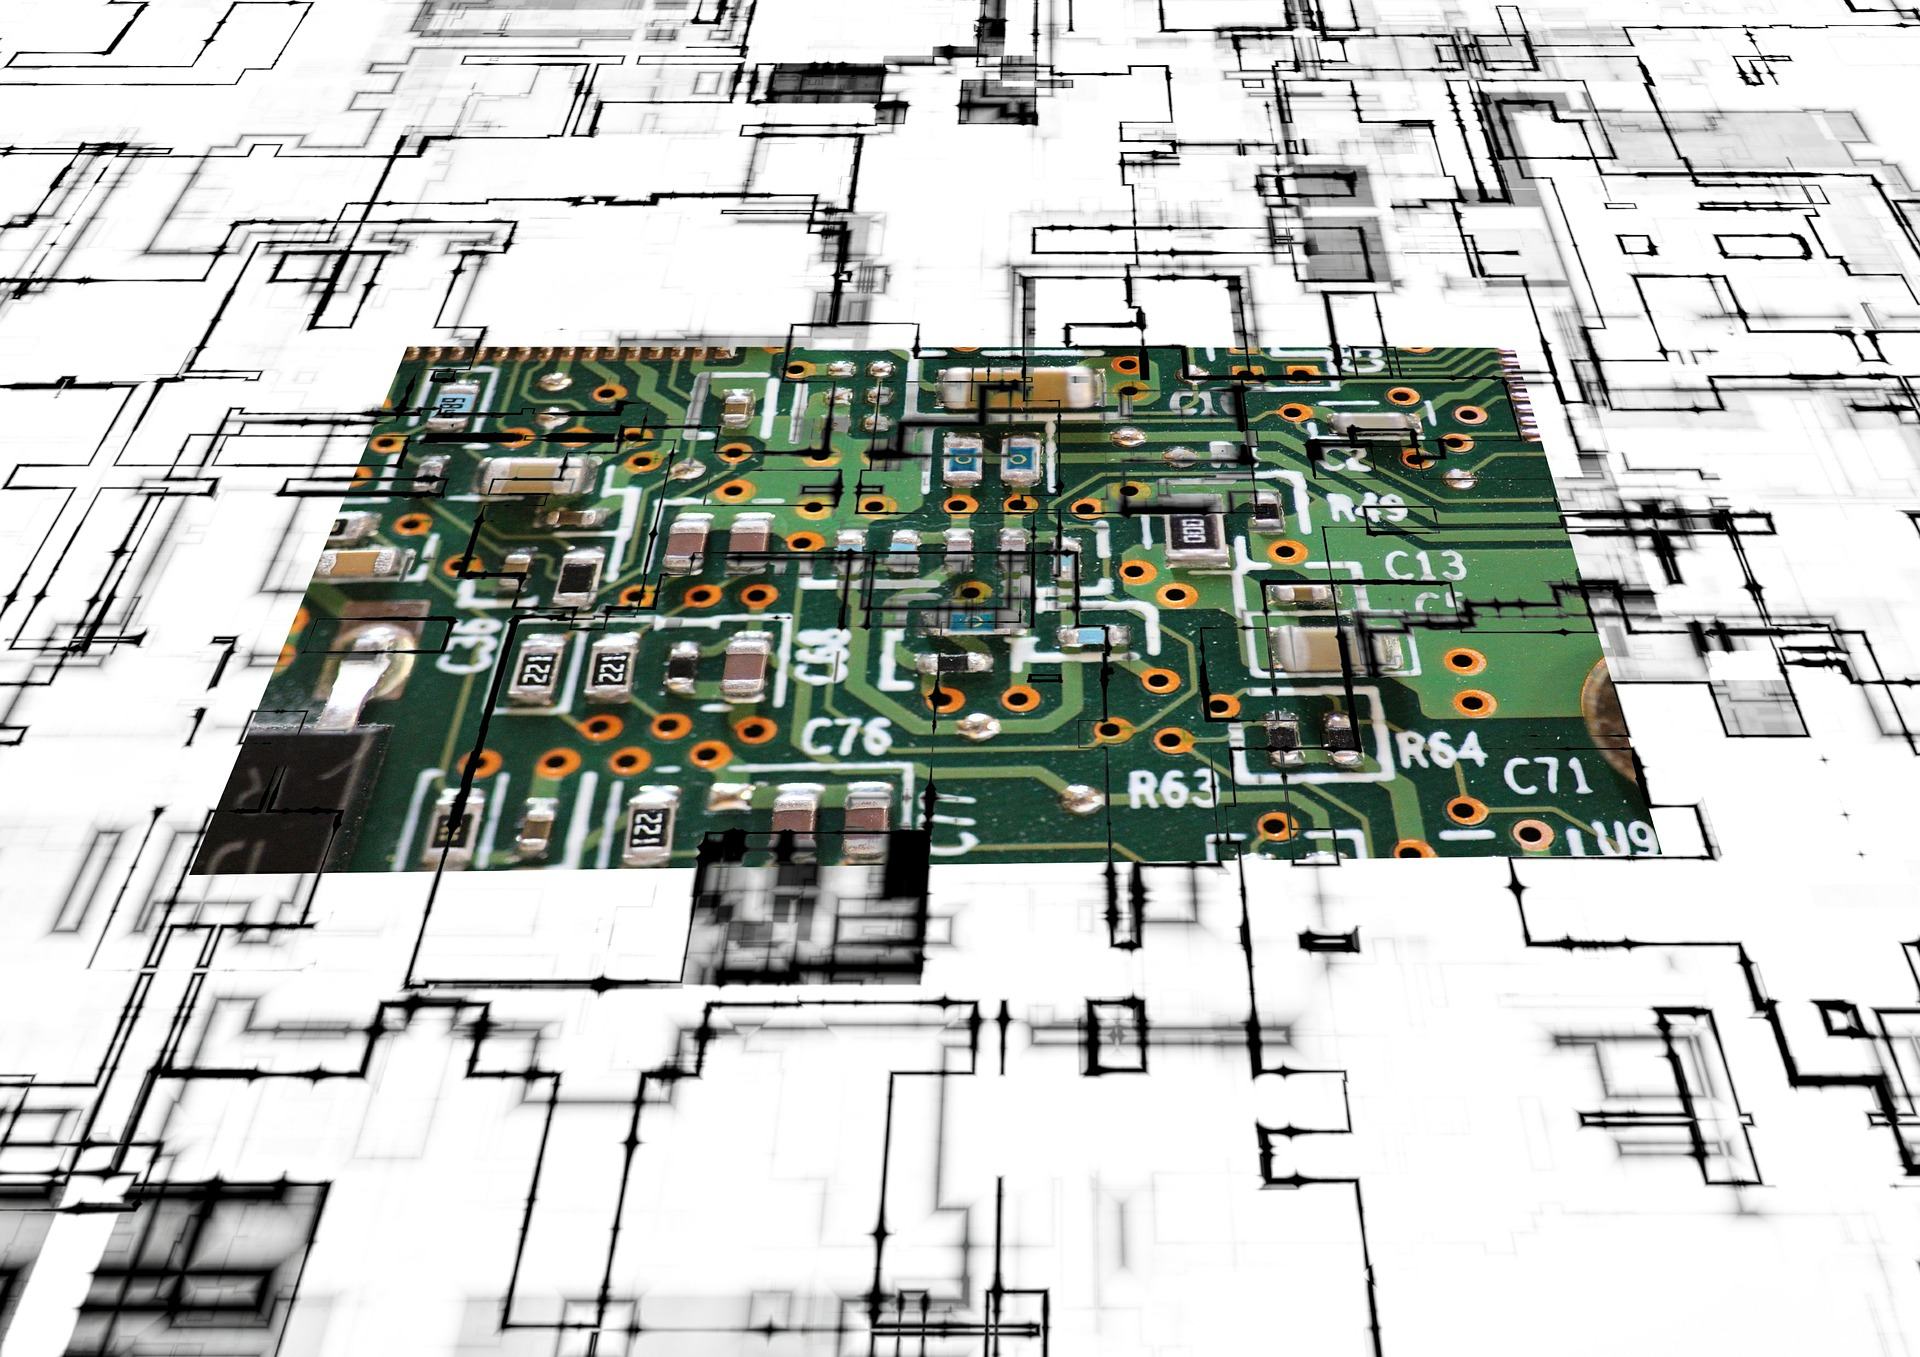
\includegraphics[width=\linewidth, trim={0 7cm 0 7cm}, clip]{board-410099_1920.jpg}}
% title graphic logo
\newcommand{\insertLogos}
{\centering \includegraphics[height=1.15cm]{TH_Logo.pdf}\hspace{1em}
\includegraphics[height=1.15cm]{Institute.jpg}}
%
% Title page of presentation
%
\makeatletter
\setbeamertemplate{title page}
{
	\vbox{}
	%
	\begin{center}
		\begin{minipage}[c]{0.8\linewidth}
			 
			\inserttitlegraphic
			    
			\begin{beamercolorbox}[sep=8pt,center]{title}
				\usebeamerfont{title}
				\inserttitle%
			\end{beamercolorbox}
			%
			\vspace{-2ex}\
			\begin{beamercolorbox}[sep=8pt,center]{author}
				\usebeamerfont{author}\small\insertauthor
				\vspace{3ex}
			\end{beamercolorbox}
			%
			\begin{minipage}[c]{.5\textwidth}
				\insertLogos
			\end{minipage}
			%
			\begin{minipage}[c]{.5\textwidth}
				\small
				
				\vspace{0.5em}
				
				\Subject\\
				
				\vspace{0.5em}
				
				\PlaceAndTime\\
				
				\vspace{0.5em}
				
				\insertinstitute
			\end{minipage}%
			%
		\end{minipage}
	\end{center}
}
\makeatother
%
% start of document
%------------------------------------------------------------------------------
\begin{document}
%
% Title page
\begin{frame}[plain]
	\titlepage
\end{frame}
%
\begin{frame}{Agenda}
	\tableofcontents
\end{frame}
%
%
\section{Introduction}
\begin{frame}{Intro}
	%
	\vfill
	Lorem ipsum dolor sit amet, consectetur adipiscing elit, sed do eiusmod tempor incididunt ut labore et dolore magna aliqua. Ut enim ad minim veniam, quis nostrud exercitation ullamco laboris nisi ut aliquip ex ea commodo consequat. Duis aute irure dolor in reprehenderit in voluptate velit esse cillum dolore eu fugiat nulla pariatur. Excepteur sint occaecat cupidatat non proident, sunt in culpa qui officia deserunt mollit anim id est laborum.
	\vfill
	%
    \begin{displayquote}
    Sé que tengo un ego del tamaño de un planeta pequeño, pero incluso yo a 
    veces me equivoco
    \end{displayquote}
	\vfill
	%
	Vel feugiat iudicabit assentior in. Sed utroque suscipiantur eu. Ad nihil dolorum accumsan est. Utroque intellegam eam ea, te pro eleifend mnesarchum.
	\vfill
	%
\end{frame}
%
\section{Topic}
%
\begin{frame}{Topic Slide 1}
	%
	\begin{columns}[totalwidth=\linewidth]
		\begin{column}{0.5\columnwidth}
			%
			Here's some text with a citation \cite{Book4}. Heres another one \cite{Book5}. Take a look at figure \ref{fig:Example} and table \ref{tab:Example}.
			\vspace{2ex}
			%
			\begin{table}[c]
				\centering
				\begin{tabular}{c|c|c}
					Object & Length & Height \\ \hline
					A      & 2.52   & 3.53   \\ \hline
					B      & 1.90   & 5.30   \\ \hline
				\end{tabular}
				\caption{Exemplary table.}
				\label{tab:Example}
			\end{table}
			%
		\end{column}
		\begin{column}{0.5\columnwidth}
			\begin{figure}
				\centering
				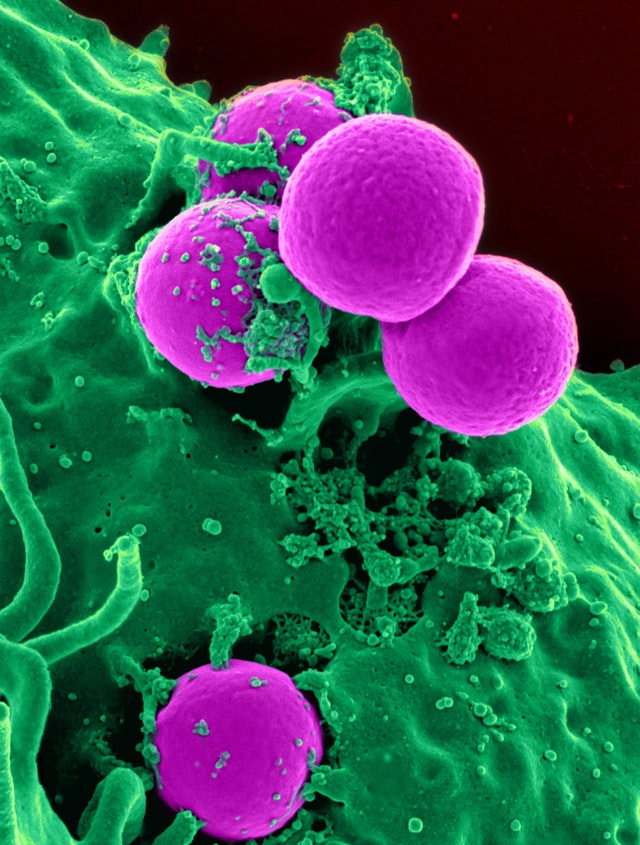
\includegraphics[height=0.5\paperheight]{pexels-pixabay-45239.jpg}
				\caption{Exemplary image. Source: \cite{PixMicroscope}}
				\label{fig:Example}
			\end{figure}    
		\end{column}
	\end{columns}
	%
\end{frame}
%
\begin{frame}{Topic Slide 2}
	%
	\begin{block}{Observation}
		This is an Observation Block.
	\end{block}
	%
	\begin{exampleblock}{Example}
		This is an Example Block.
	\end{exampleblock}
	%
	\begin{alertblock}{Alert}
		This is an Alert Block.
	\end{alertblock}
	%
	\vfill
	This leads to the following equation:
	\begin{equation}
		M = \frac{2\pi}{x^5 - y^3 + \sin(x)} \cdot \int_{a}^{b} f(x)^2 \,dx
	\end{equation}
\end{frame}
%
%
\section{Outlook}
\begin{frame}{Outlook}
	%
	\textbf{List}\\
	\begin{itemize}
		\item Pri sonet labore expetenda
		      \begin{itemize}
		      	\item Svix te wisi atqui inermis
		      	\item  Cum dolor delenit argumentum et
		      \end{itemize}
		\item no vim quidam probatus senserit
		\item accommodare necessitatibus ad quo
		\item integre persecuti efficiantur at pro
	\end{itemize}
	%
	\vfill
	%
	\textbf{List 2}\\
	\begin{enumerate}
		\item no vis patrioque reprehendunt
		\item partem definitiones nam
		\item vel wisi dignissim voluptatibus ut
	\end{enumerate}
	%
\end{frame}
%
%------------------------------------------------------------------------------
%
\section{Sources}
%
\begin{frame}{Sources (1)}
	\textbf{Image Sources}\\[2ex]
	\small Title page:
	\fullcite{PixBoard}
	\vspace{2ex}
	
	\printbibliography[keyword=pic]
\end{frame}
%
\begin{frame}
	\frametitle{Sources (2)}
	\textbf{Sources}\\
	\printbibliography[keyword=inf]
	\vfill
	%
	\textbf{Additional Literature}
	\small
	\begin{itemize}
		\item \fullcite{Book1}
		\item \fullcite{Book2}
		\item \fullcite{Book3}
	\end{itemize}
\end{frame}
%
\begin{frame}{}
	\usebeamerfont{AAA}
	\begin{center}
		\Large Thank you for your attention\\[2ex] 
		\small Please feel free to ask any questions
		\vspace{10ex}
		
		Contact:\\
		\Contactmail
	\end{center}
\end{frame}
%
%------------------------------------------------------------------------------
\end{document}